
\begin{frame}{Trækjagt}
    
    \begin{columns}[T]
        \begin{column}{0.58\textwidth}
            \begin{itemize}
                \item Passiv jagtform - venter på trækkende fugle
                \item Solo eller få jægere sammen
                \item Der anvendes skjul, camouflage og lokkefugle
                \item Meget udbredt jagtform i DK
                \item Der anvendes haglgevær
                \item Der anvendes apporterende hunde (lovkrav)
            \end{itemize}
        \end{column}
        
        \begin{column}{0.4\textwidth}
            \centering
            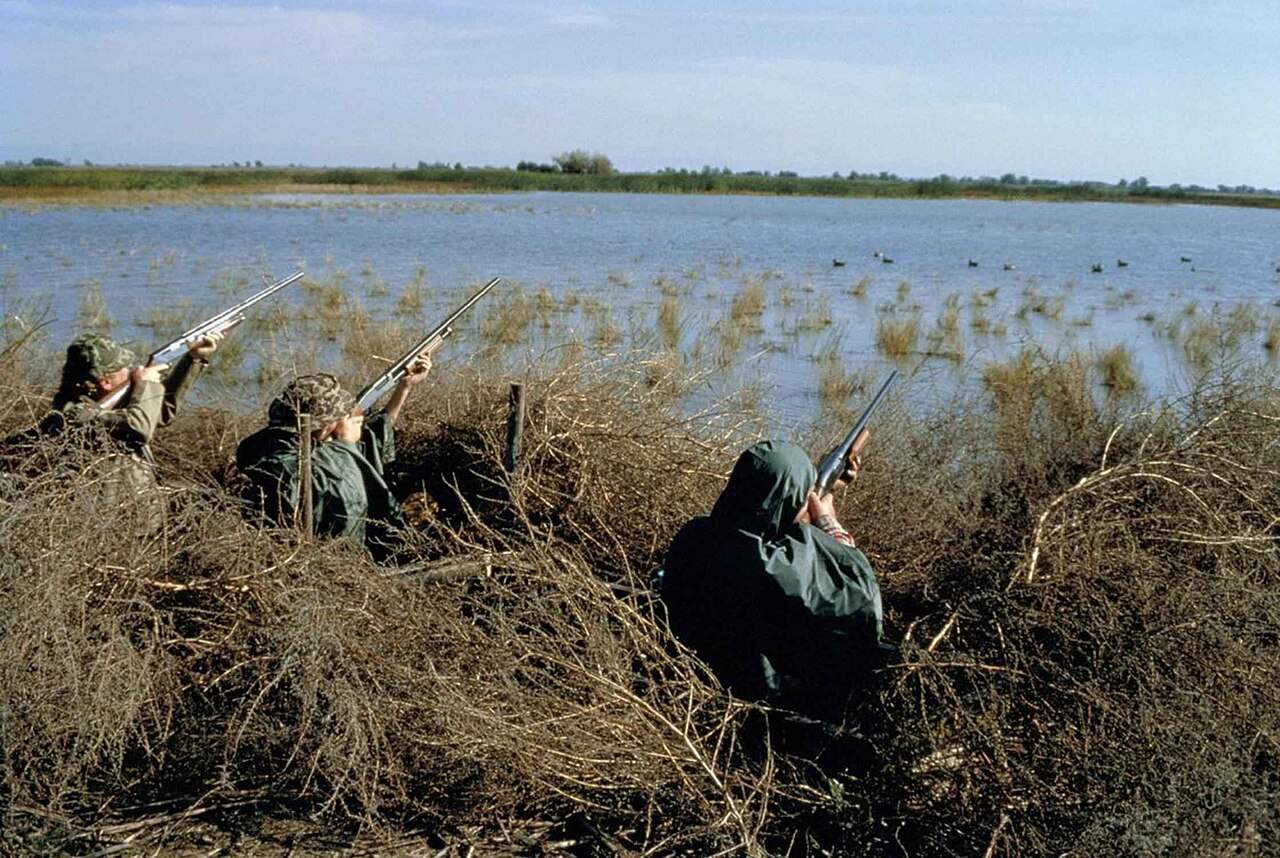
\includegraphics[width=\textwidth,height=0.85\textheight,keepaspectratio]
                {Billeder/Jagtformer/traekjagt_01}
            % Alternativt brug en af disse stilrene billeder:
            % \includegraphics[width=\textwidth]{highseat-snow-forest-hunter.jpg}
            % \includegraphics[width=\textwidth]{hunter-leaning-tree-rifle.jpg}
        \end{column}
    \end{columns}
    
\end{frame}